\chapter{Конструкторский раздел}

\section{IDEF0--диаграммы}
На рисунках \ref{fig:idef0-1}--\ref{fig:idef0-2} приведены диаграммы, описывающие последовательность действий, выполняемых в ПО.

\begin{figure}[h!btp]
	\centering
	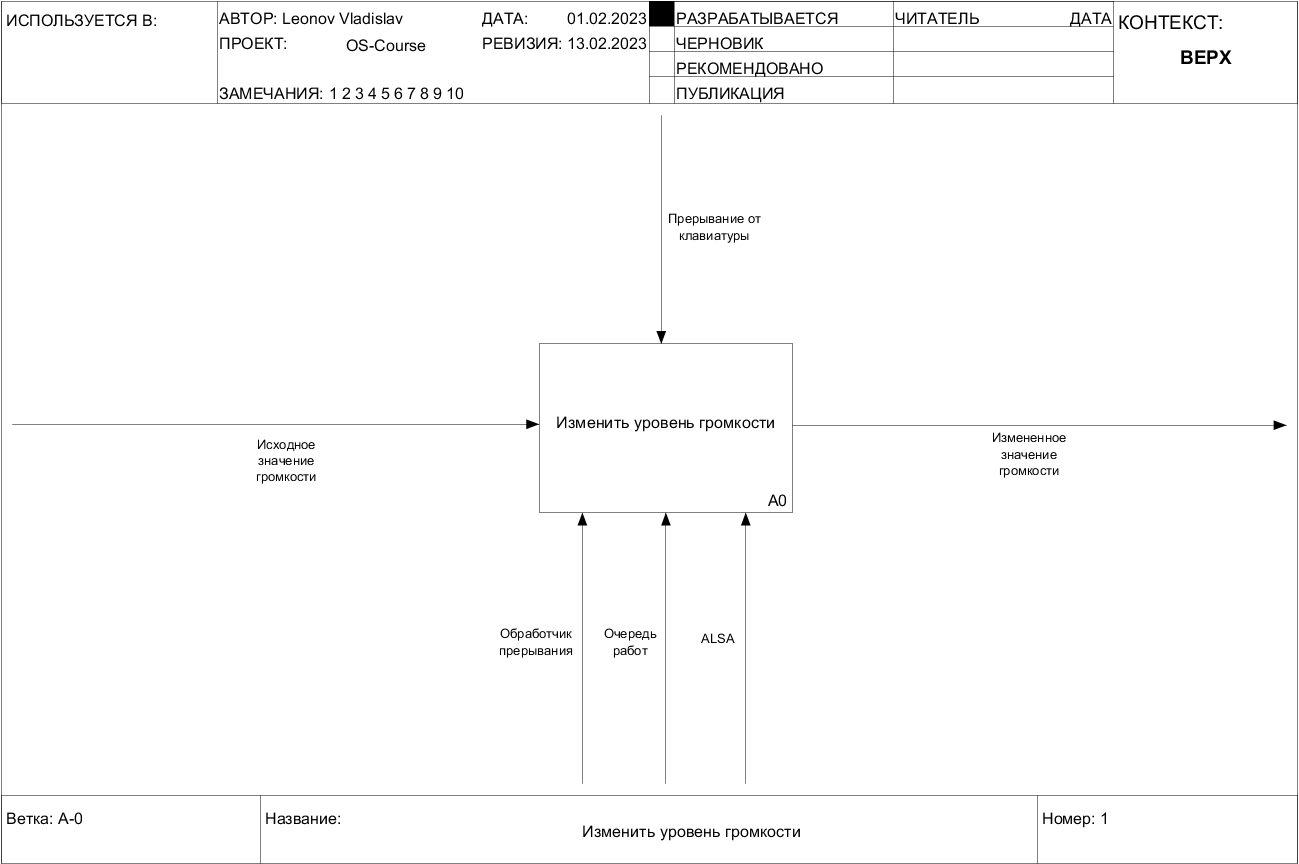
\includegraphics[scale = 0.35]{inc/img/01_A-0.png}
	\caption{Уровень А0}
	\label{fig:idef0-1}	
\end{figure}

\clearpage

\begin{figure}[h!btp]
	\centering
	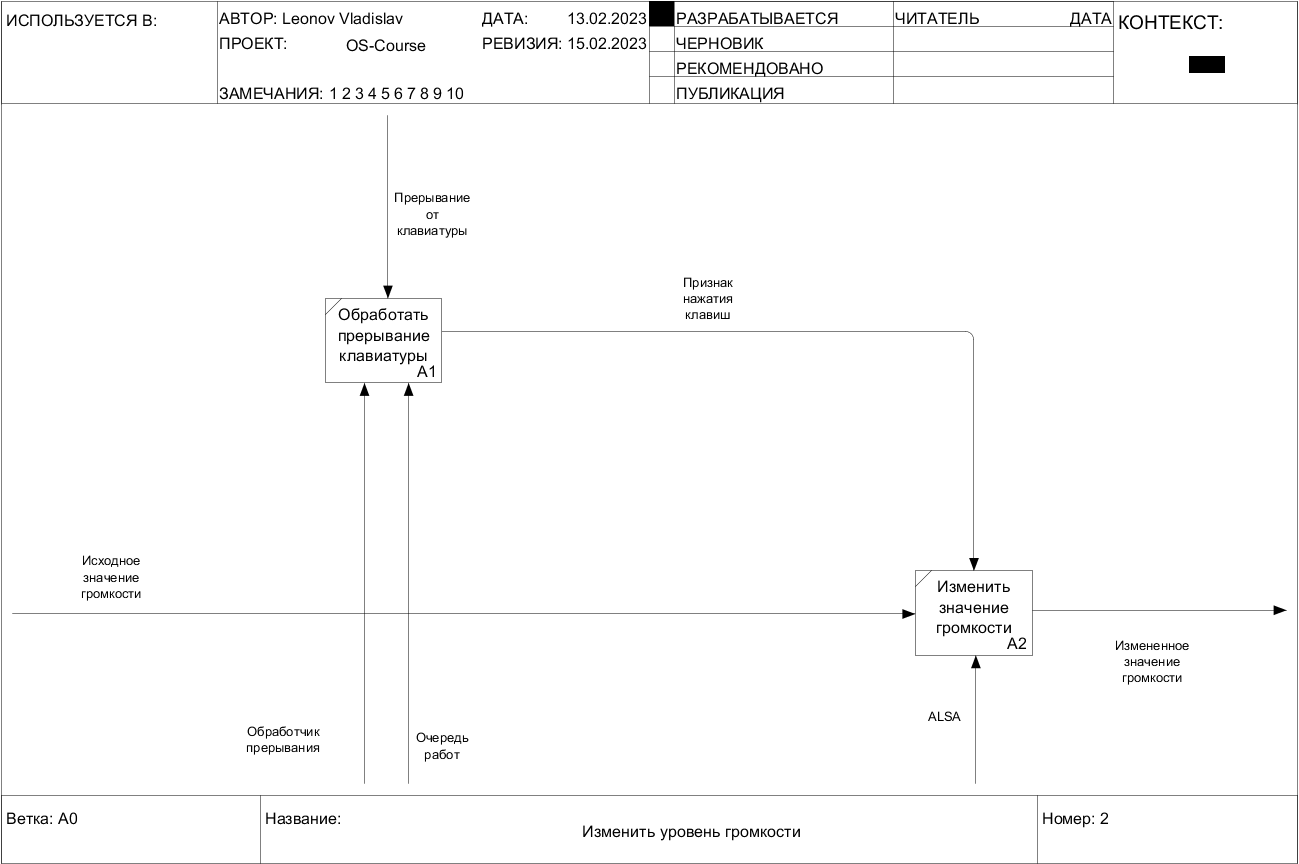
\includegraphics[scale = 0.35]{inc/img/02_A0.png}
	\caption{Уровень А1-A2}
	\label{fig:idef0-2}	
\end{figure}

\section{Разработка алгоритмов}

Одновременное нажатие следующих клавиш выполняет следующие действия:
\begin{itemize}
    \item ALT и 0 --- установить уровень громкости $0\%$; 
    \item ALT и 1 --- установить уровень громкости $10\%$; 
    \item ALT и 2 --- установить уровень громкости $20\%$; 
    \item ALT и 3 --- установить уровень громкости $30\%$; 
    \item ALT и 4 --- установить уровень громкости $40\%$; 
    \item ALT и 5 --- установить уровень громкости $50\%$; 
    \item ALT и 6 --- установить уровень громкости $60\%$; 
    \item ALT и 7 --- установить уровень громкости $70\%$; 
    \item ALT и 8 --- установить уровень громкости $80\%$; 
    \item ALT и 9 --- установить уровень громкости $90\%$; 
    \item ALT и -- --- уменьшить текущий уровень громкости на 1\%;
    \item ALT и = --- увеличить текущий уровень громкости на 1\%.     
\end{itemize}

Алгоритм обработки прерывания от клавиатуры изображен на рисунке \ref{fig:kb_handler}.
\begin{figure}[h!btp]
	\centering
	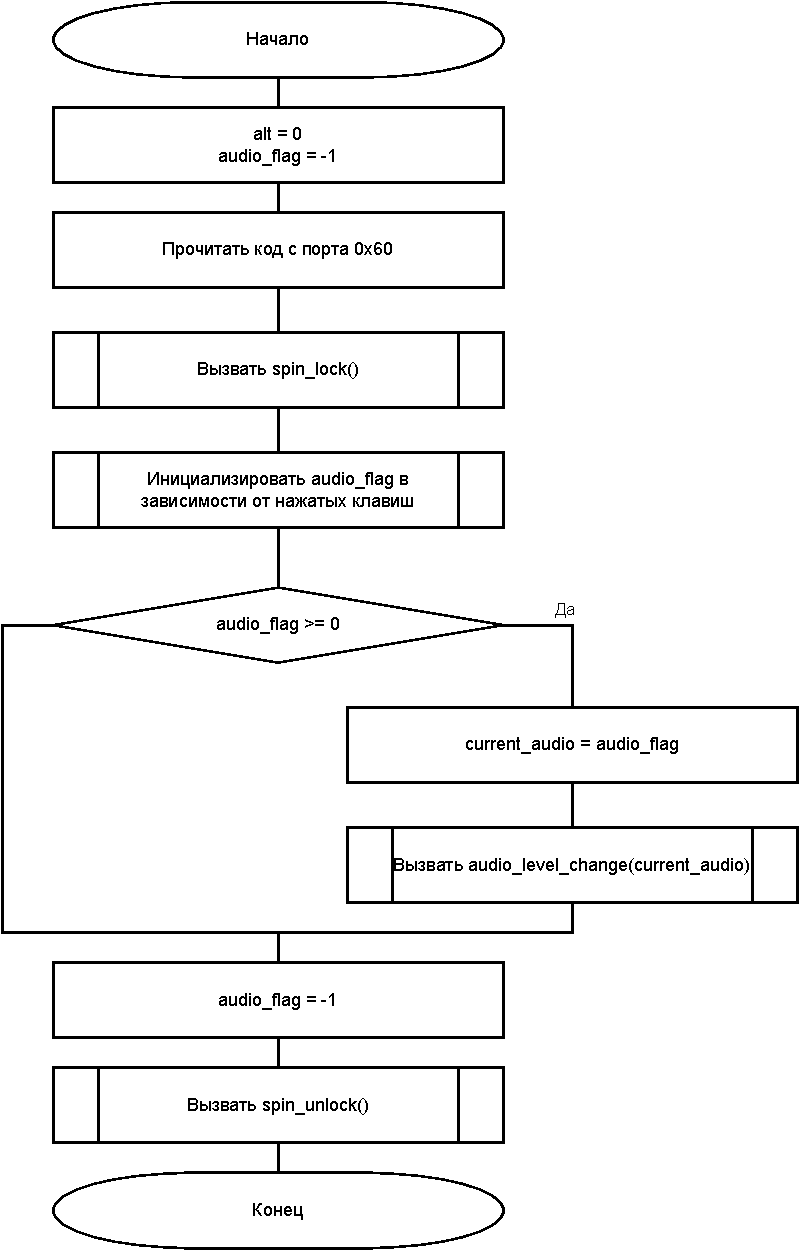
\includegraphics[scale = 0.9]{inc/diag/kb_handler.pdf}
	\caption{Алгоритм обработки прерывания от клавиатуры}
	\label{fig:kb_handler}	
\end{figure}

\clearpage

Алгоритм изменения громкости изображен на рисунке \ref{fig:volume_controller}.
\begin{figure}[h!btp]
	\centering
	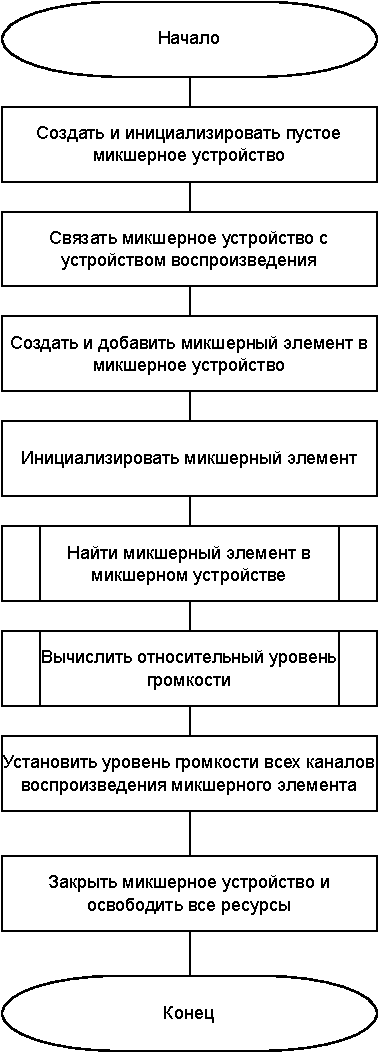
\includegraphics[scale = 1.3]{inc/diag/audio_controller.pdf}
	\caption{Алгоритм изменения громкости}
	\label{fig:volume_controller}	
\end{figure}

\clearpage

\section{Структура ПО}

Разработанное программное обеспечение включает в себя:
\begin{itemize}
    \item загружаемый модуль ядра, осуществляющий перехват прерываний от клавиатуры;
    \item вспомогательный модуль для регулировки громкости.
\end{itemize}

 На рисунке \ref{fig:module_struct} приведена структура ПО.
 \begin{figure}[h!btp]
	\centering
	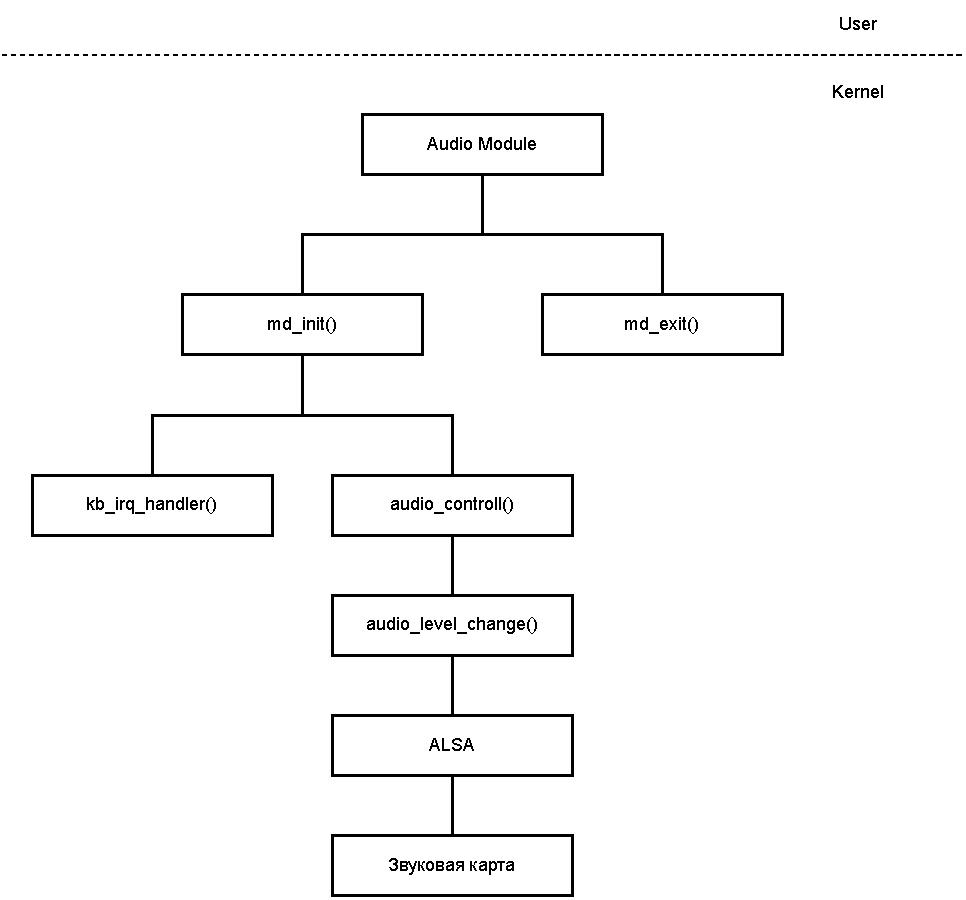
\includegraphics[scale = 1]{inc/diag/module_struct.pdf}
	\caption{Структура ПО}
	\label{fig:module_struct}	
\end{figure}

